Tú tiene una constructora que busca comprar un terreno para construir un fraccionamiento.

Actualmente, el gobierno de Karelopolis permite que compres un terreno en la región para desarrollo. La región para desarrollo se ve como una cuadricula de \(N\) filas y \(M\) columnas. El terreno que compres debe ser rectangular y alineada a la cuadricula, es decir, no puedes comprar una celda de la cuadricula de forma incompleta.

Además, tu calculaste cuanto dinero obtendrías si compras cada celda, en concreto, la celda que esta en la fila \(i\) y columna \(j\) aportaría \(v_{ij}\) pesos. Como hay celdas con valor positivo y otras con valor negativo, te preguntas cual es el máximo valor que puedes obtener.

Por ejemplo, si la región para desarrollo se ve de la siguiente forma:

\begin{center}
	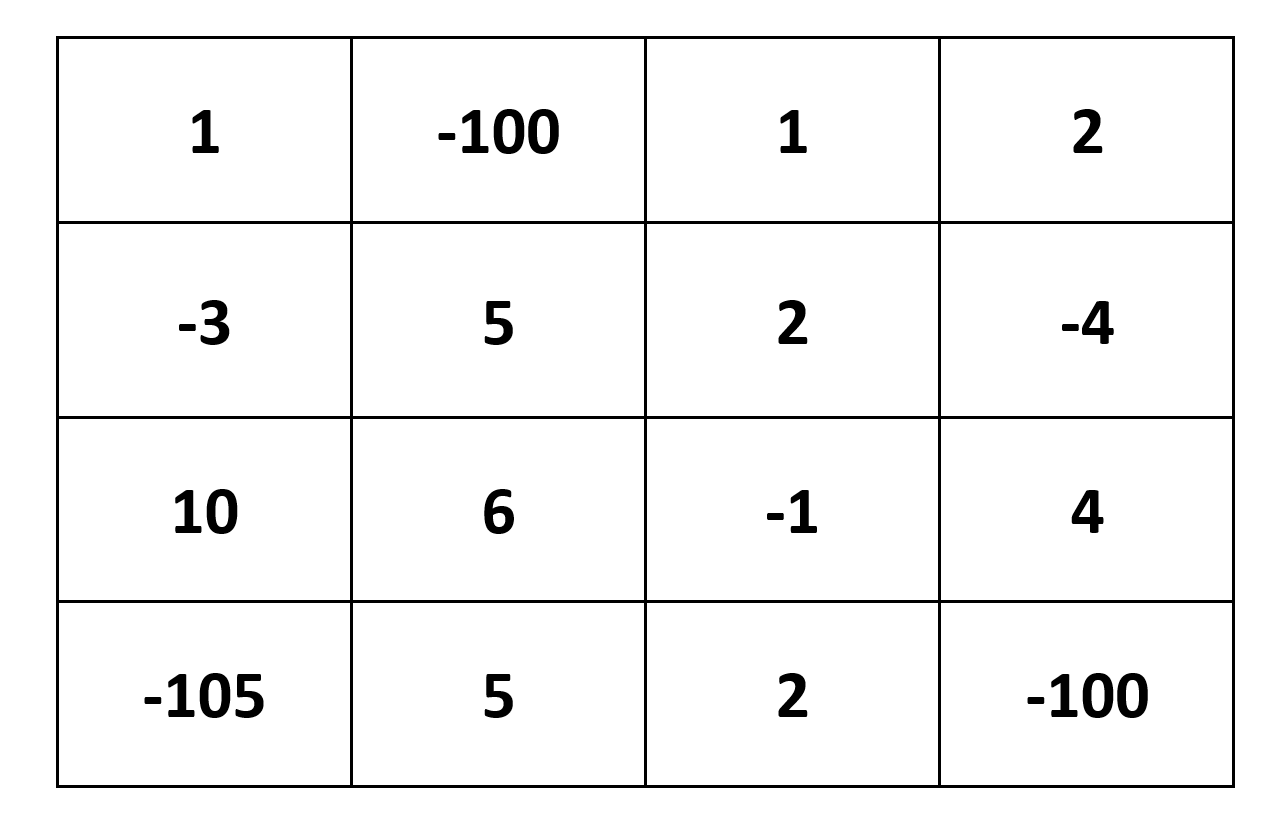
\includegraphics[scale=0.15]{terrenos}
\end{center}

Tu puedes obtener hasta 19 pesos comprando el terreno:

\begin{center}
	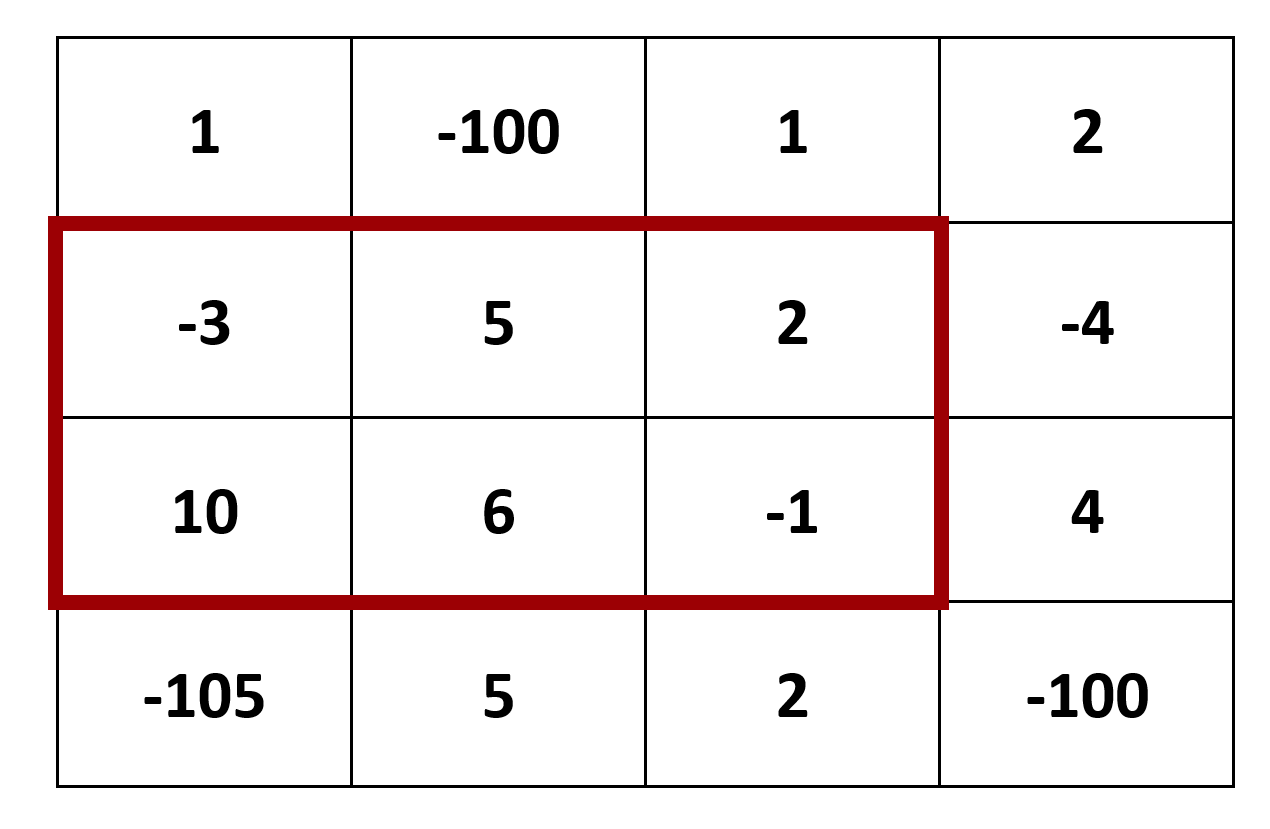
\includegraphics[scale=0.15]{terrenos2}
\end{center}


Encuentra el máximo valor posible si compras un terreno dada la región para desarrollo.

\subsubsection*{Entrada}

En la primera línea recibes \(N\) y \(M\).

En las siguientes \(N\) líneas recibirás \(M\) enteros representando los valores de \(v_{ij}\).

\subsubsection*{Salida}

Un entero que sea el mayor valor de un terreno.

\subsubsection*{Ejemplo}

\begin{casebox2}
	\scase{
		4 4\\
		1 -100 1 2\\
		-3 5 2 -4\\
		10 6 -1 4\\
		-105 5 2 -100
	}{19}
	\hline
\end{casebox2}

\subsubsection*{Límites}

\begin{plimits}
	\item \(1\leq N, M\leq 75 \)
	\item \(-10^9\leq v_{ij}\leq 10^9 \)
\end{plimits}

\subsubsection*{Subtareas}

\begin{plimits}
	\item (40 pts) \(1\leq N, M\leq 15 \)
	\item (60 pts) Sin consideraciones extra.
\end{plimits}
